\section{Extensión del método al Dominio de $\mathbb{C}$}

El teorema fundamental del álgebra enuncia lo siguiente:

\begin{theorem}
 Todo polinomio de grado n $n \geq 1$ tiene n raíces complejas
\end{theorem}

Cuya demostración se puede encontrar en \cite{lankham}

A partir de esto, podemos expandir la búsqueda de raíces incluyendo números imaginarios y pasar del plano exclusivamente real, al plano complejo  $\mathbb{C}$ y extender a su vez el método de Newton-Raphson, cuya única modificación será que ahora es capaz de recibir funciones complejas y puntos iniciales del mismo tipo

\begin{equation}
     z = z_{n-1} - \frac{f(z_{n-1})}{f'(z_{n-1})}
\end{equation}

Por ejemplo, sea $f(z) = z^2+1, f'(z) = 2z$, veremos que obtenemos las  raíces $-i,i$ con la siguiente imagen de sus puntos de convergencia
\begin{figure}[H]
    \centering
    
\includegraphics{images/eq3-1.png}
    \caption{ Zonas de convergencia de $ x^2+1$}
    \label{fig:eq_cuad_compleja_1}
\end{figure}

y si colocamos el mapa de la rapidez de convergencia de sus puntos (Los colores más claros indican mayor cantidad de iteraciones)
\begin{figure}[H]
    \centering
    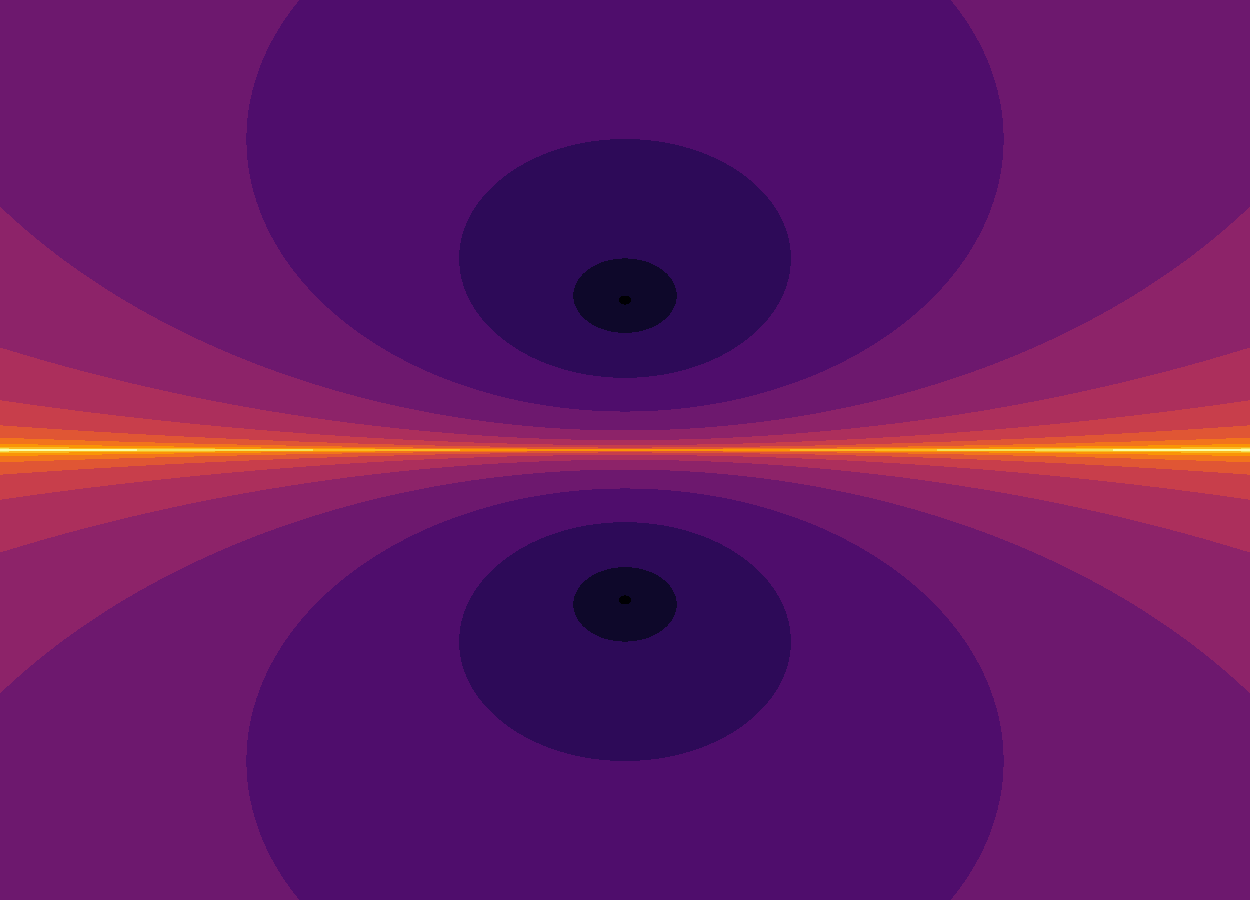
\includegraphics[scale=0.26]{images/eq3-2.png}
    \caption{Rapidez de convergencia de los puntos de $ x^2+1$}
    \label{fig:eq_cuad_compleja_2}
\end{figure}
Comportándose muy similar a la función vista previamente en Figura \ref{fig:eq_cuadratica_2}, con la división siendo en este caso el eje de los reales 

Pero que pasa con funciones de grado $n \geq 2$
Si observamos la función $f(z) = z^3-1$, obtenemos las raíces $(-0.5,-0.866i),(-0.5+0.866i),(1+0i)$ y al generar su mapa de convergencia, obtenemos la siguiente imagen, la cual genera un patrón interesante
\begin{figure}[H]
    \centering
    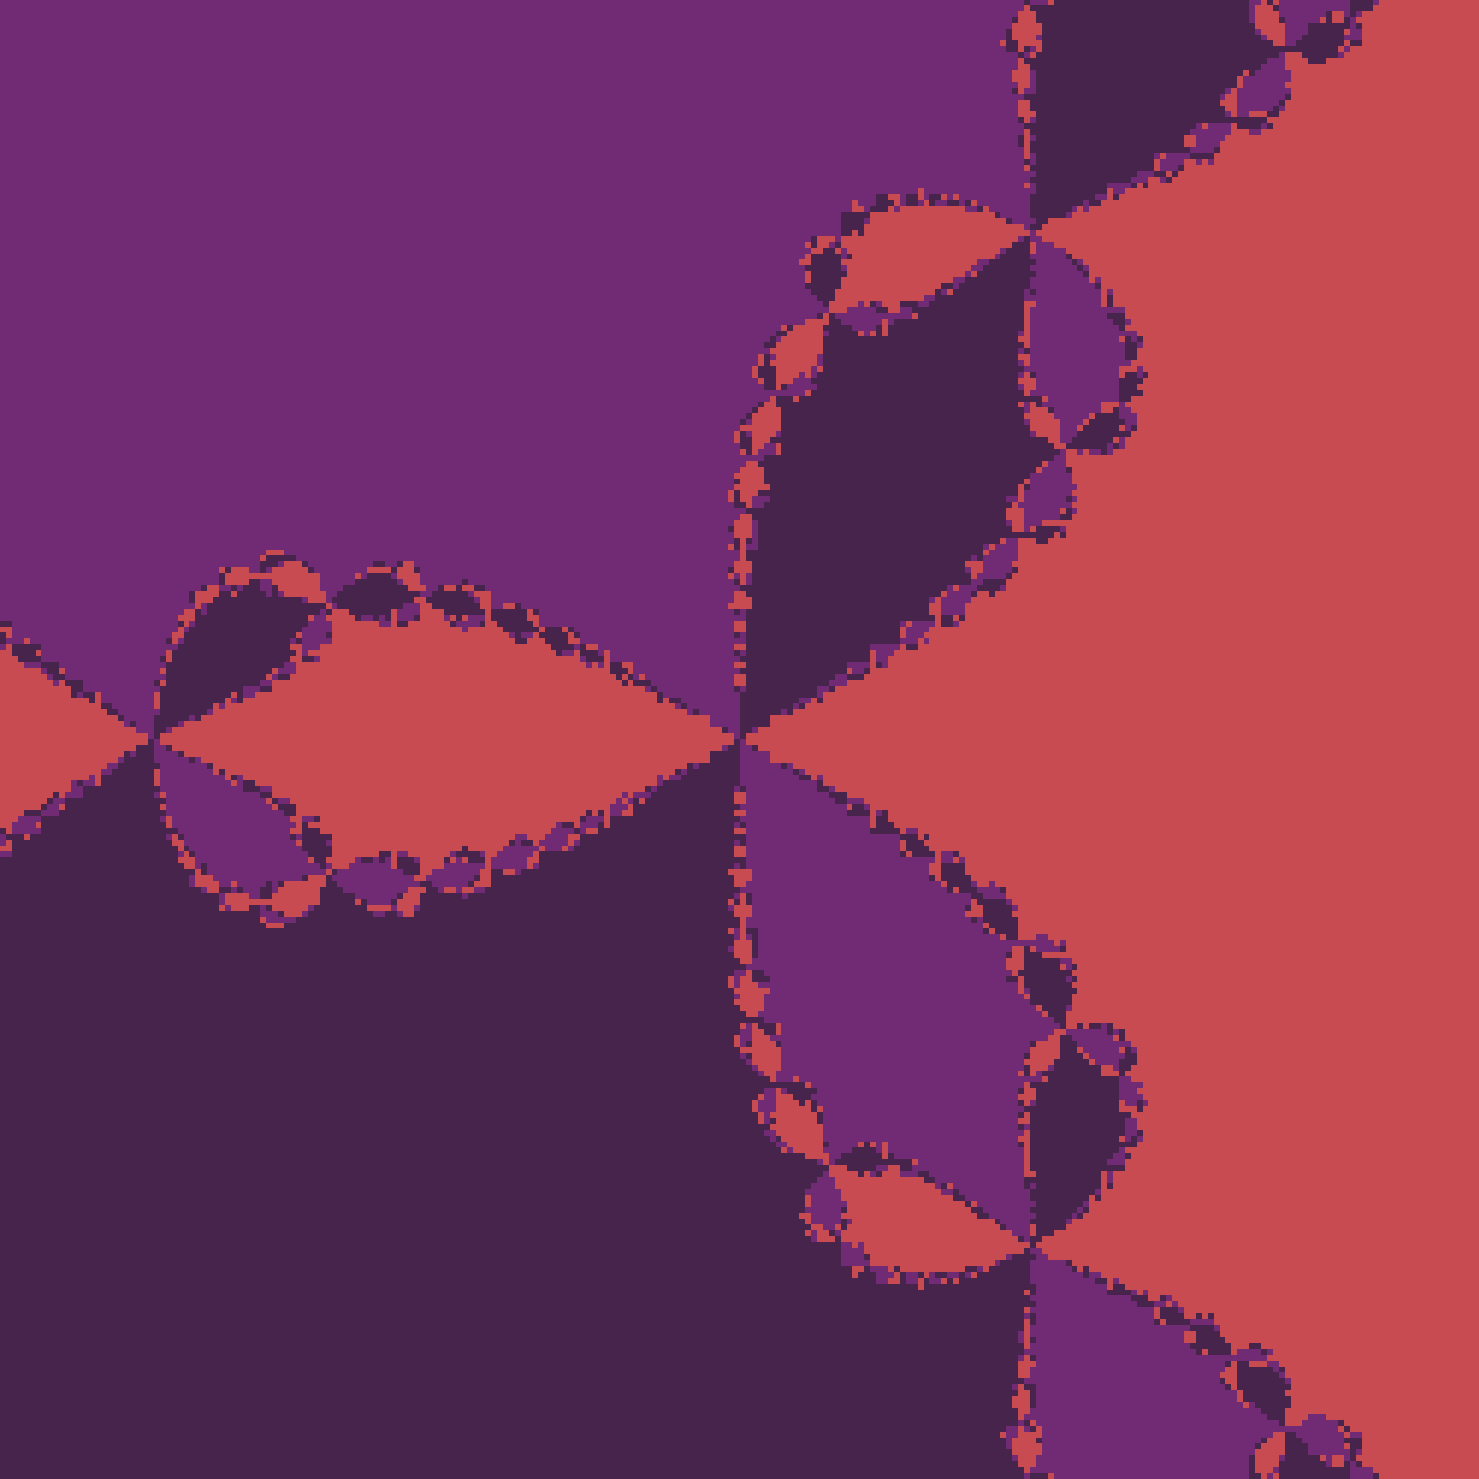
\includegraphics{images/eq4-1.png}
    \caption{Zonas de convergencia de los puntos de $ x^3-1$}
    \label{fig:eq_cub_compleja_1}
\end{figure}
y si se gráfica de la rapidez de convergencia de sus puntos vemos lo siguiente
\begin{figure}[H]
    \centering
    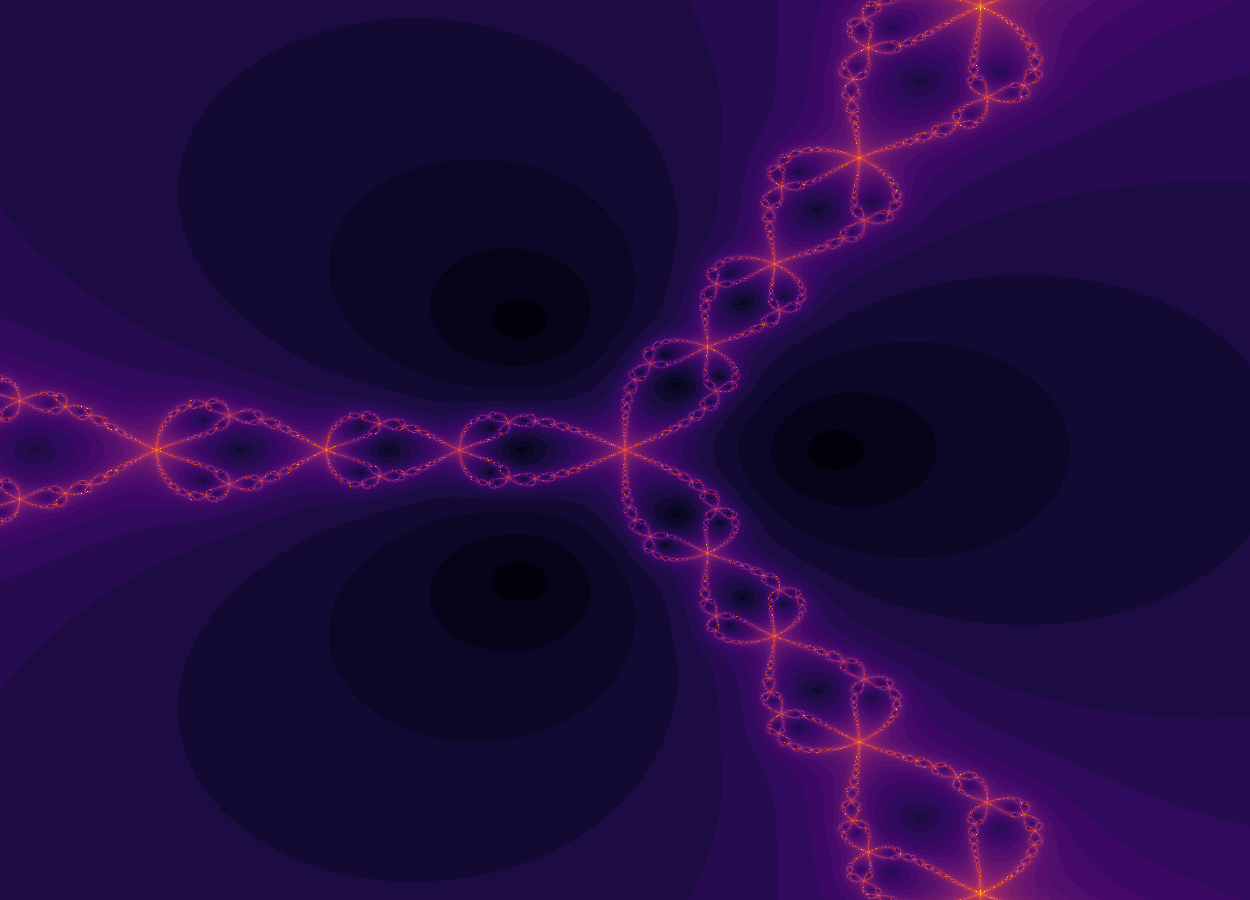
\includegraphics[scale=0.26]{images/eq4-2.png}
    \caption{Rapidez de convergencia de los puntos de $ x^3-1$}
    \label{fig:eq_cub_compleja_2}
\end{figure}
Aquí notamos dos comportamientos inusuales
El primero de ellos es que se forma un fractal muy similar a un conjunto de Julia\cite{badger}, y que se empezaba a vislumbrar en la Figura \ref{fig:eq_cuadratica_2}, donde cerca de los bordes donde comenzaría la siguiente región de otra raíz, observamos una formación que, sin importar el nivel de acercamiento que se le de, contiene colores correspondientes a otras zonas de atracción, los cuales a su vez contienen más de estas zonas de atracción de las demás raíces. Estos fractales son conocidos como fractales de Newton \cite{3b1b}

Podemos ver en esto que se réplica la idea de que entre regiones donde el método tomaría muchas iteraciones o donde fallase, se ven contenidas zonas de atracción hacia las demás raíces, pero además podemos observar que cada zona es dividida entre lugares donde todos los puntos convergen hacia una única raíz o lugares donde se contienen n colores divididos de manera recursiva en estas dos zonas

Además se puede apreciar, como ya se mencionaba, que existen zonas, cerca de los bordes y de los puntos críticos, donde los valores de puntos iniciales tomados de dicho sitio tomarán una gran cantidad de iteraciones en converger, como puede verse en \ref{fig:eq_cubica_1}, extendiendo el comportamiento visto dentro de los reales con al función $x^3-x$.

Dichos comportamientos pueden verse en funciones de mayor grado, como puede verse en los ejemplos ilustrados de la sección correspondiente